\documentclass[11pt,a4paper]{article}

% ============================================
% PACKAGES
% ============================================
\usepackage[utf8]{inputenc}
\usepackage[T1]{fontenc}
\usepackage{lmodern}
\usepackage[margin=1in]{geometry}
\usepackage{xcolor}
\usepackage{hyperref}
\usepackage{graphicx}
\usepackage{booktabs}
\usepackage{longtable}
\usepackage{enumitem}
\usepackage{fancyhdr}
\usepackage{titlesec}
\usepackage{tcolorbox}
\usepackage{listings}
\usepackage{tikz}
\usetikzlibrary{shapes.geometric, arrows.meta, positioning, fit, backgrounds}

% ============================================
% COLORS
% ============================================
\definecolor{ericssonblue}{RGB}{0, 130, 180}
\definecolor{quantumpurple}{RGB}{102, 51, 153}
\definecolor{telecomgray}{RGB}{70, 70, 70}
\definecolor{successgreen}{RGB}{46, 125, 50}
\definecolor{warningorange}{RGB}{230, 126, 34}
\definecolor{dangerred}{RGB}{192, 57, 43}
\definecolor{lightbg}{RGB}{248, 249, 250}

% ============================================
% HYPERREF SETUP
% ============================================
\hypersetup{
    colorlinks=true,
    linkcolor=ericssonblue,
    urlcolor=quantumpurple,
    citecolor=telecomgray,
    pdftitle={TELEQUM v2.0 Implementation Plan},
    pdfauthor={Abdulmalek Baitulmal},
    pdfsubject={Quantum-Telecom Platform Evolution}
}

% ============================================
% HEADERS & FOOTERS
% ============================================
\pagestyle{fancy}
\fancyhf{}
\fancyhead[L]{\textcolor{telecomgray}{\textsc{TELEQUM v2.0}}}
\fancyhead[R]{\textcolor{telecomgray}{\textsc{Implementation Plan}}}
\fancyfoot[C]{\thepage}
\renewcommand{\headrulewidth}{0.4pt}

% ============================================
% TITLE FORMATTING
% ============================================
\titleformat{\section}
{\color{ericssonblue}\normalfont\Large\bfseries}
{\thesection}{1em}{}

\titleformat{\subsection}
{\color{quantumpurple}\normalfont\large\bfseries}
{\thesubsection}{1em}{}

% ============================================
% CUSTOM BOXES
% ============================================
\newtcolorbox{importantbox}{
    colback=warningorange!10,
    colframe=warningorange,
    fonttitle=\bfseries,
    title=Important Decision Required,
    arc=3mm
}

\newtcolorbox{warningbox}{
    colback=dangerred!10,
    colframe=dangerred,
    fonttitle=\bfseries,
    title=Breaking Change Warning,
    arc=3mm
}

\newtcolorbox{successbox}{
    colback=successgreen!10,
    colframe=successgreen,
    fonttitle=\bfseries,
    title=Success Criteria,
    arc=3mm
}

% ============================================
% CODE LISTINGS
% ============================================
\lstset{
    basicstyle=\ttfamily\small,
    backgroundcolor=\color{lightbg},
    frame=single,
    rulecolor=\color{telecomgray!50},
    breaklines=true,
    columns=fullflexible
}

% ============================================
% DOCUMENT START
% ============================================
\begin{document}

% ============================================
% TITLE PAGE
% ============================================
\begin{titlepage}
    \centering
    \vspace*{2cm}
    
    {\Huge\bfseries\textcolor{ericssonblue}{TELEQUM v2.0}\par}
    \vspace{0.5cm}
    {\LARGE\textcolor{quantumpurple}{From Personal Testbed to Industrial-Grade Platform}\par}
    
    \vspace{1.5cm}
    
    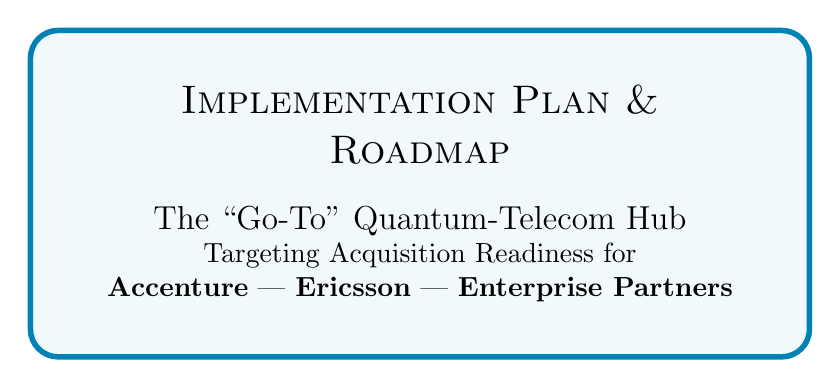
\begin{tikzpicture}
        \node[draw=ericssonblue, line width=2pt, rounded corners=10pt, 
              inner sep=20pt, fill=ericssonblue!5] {
            \begin{minipage}{0.7\textwidth}
                \centering
                \Large\textsc{Implementation Plan \& Roadmap}\\[10pt]
                \large The ``Go-To'' Quantum-Telecom Hub\\
                \normalsize Targeting Acquisition Readiness for\\
                \textbf{Accenture} | \textbf{Ericsson} | \textbf{Enterprise Partners}
            \end{minipage}
        };
    \end{tikzpicture}
    
    \vspace{2cm}
    
    \begin{tabular}{ll}
        \textbf{Author:} & Abdulmalek Baitulmal \\
        \textbf{Role:} & Quantum Strategy Lead (MENA Region) \\
        \textbf{Date:} & January 27, 2026 \\
        \textbf{Version:} & 2.0-DRAFT \\
    \end{tabular}
    
    \vspace{1cm}
    
    \begin{minipage}{0.8\textwidth}
        \centering
        \textit{``Bridge between Telecom Legacy Systems and Quantum Futures''}
    \end{minipage}
    
    \vfill
    
    \href{https://github.com/Abdulmalek-HoM/telequm}{\texttt{github.com/Abdulmalek-HoM/telequm}}\\[5pt]
    \href{https://www.linkedin.com/in/abdulmalek-baitulmal-543753140/}{LinkedIn: Abdulmalek Baitulmal}
    
\end{titlepage}

% ============================================
% TABLE OF CONTENTS
% ============================================
\tableofcontents
\newpage

% ============================================
% EXECUTIVE SUMMARY
% ============================================
\section{Executive Summary}

\subsection{Strategic Objective}
Transform TELEQUM from a portfolio-style collection of workshops and notebooks into the ``Go-To'' \textbf{Quantum-Telecom Hub} that positions itself as an acquisition target for enterprise players like \textbf{Accenture} and \textbf{Ericsson}.

\subsection{Key Differentiators}
\begin{itemize}
    \item \textbf{VQE/QAOA optimization for 6G} --- Proven implementations with industrial ROI
    \item \textbf{QEM-Former} --- Graph Transformer for Quantum Error Mitigation
    \item \textbf{IET-published framework} for national quantum adoption (MENA focus)
    \item \textbf{IEEE ComSoc} workshop delivery experience
\end{itemize}

\subsection{Target Audience}
\begin{itemize}
    \item VP of Engineering at Ericsson
    \item Managing Director at Accenture Qatar
    \item Telecom operators seeking quantum readiness
    \item ICT Engineers upskilling in quantum technologies
\end{itemize}

% ============================================
% CURRENT STATE ANALYSIS
% ============================================
\section{Current State Analysis (v1.1)}

\subsection{Repository Structure}

The current TELEQUM repository follows a \textbf{``Portfolio Style''} organization, structured around specific events and presentations rather than domain knowledge areas.

\begin{lstlisting}[caption={Current v1.1 Directory Structure}]
telequm/
├── .ipynb_checkpoints/
├── IEEE-ComSoc Workshop/           # Event-specific (9 notebooks)
│   ├── Quantum Computing Basics - ComSoc V2.ipynb
│   ├── Section 1 - Bell State Creation.ipynb
│   ├── Section 2 - Quantum in Telecommunications.ipynb
│   ├── Section 3 - Quantum Fourier Transform.ipynb
│   └── ...
├── QCoffee Corner; The Quantum Heist/   # Event-specific (8 files)
│   ├── Quantum_Heist_V1-V6.ipynb variants
│   └── Telegram Packets All.json (70MB!)
├── Quantum Computing for 6G and Beyond/ # Domain content (5 notebooks)
│   ├── 04_1_6G_Network_Optimization_with_QAOA.ipynb
│   ├── 04_2_6G_Advanced_Resource_Allocation_with_VQE.ipynb
│   ├── 04_3_6G_Intelligent_Beamforming_with_QML.ipynb
│   └── 04_3.2_Classical_Implementation.ipynb
├── Saraya Hamra Uni/                # Event-specific (2 notebooks)
├── Post-Quantum Cryptography (PQC)/ # EMPTY
├── Quantum Cryptography (QKD)/      # EMPTY
├── Quantum Internet (Quantum Networks)/ # EMPTY
├── Quantum Sensing and Metrology.../    # EMPTY
└── README.md
\end{lstlisting}

\subsection{Critical Issues Identified}

\begin{longtable}{p{5cm}p{6cm}p{2cm}}
\toprule
\textbf{Issue} & \textbf{Impact} & \textbf{Priority} \\
\midrule
\endhead
Event-based organization (IEEE, QCoffee, Saraya) & Fragments domain knowledge across events & \textcolor{dangerred}{High} \\
README describes aspirational structure & Confusion for new contributors & \textcolor{dangerred}{High} \\
4 planned directories are empty & Platform appears incomplete & \textcolor{dangerred}{High} \\
No \texttt{requirements.txt} or \texttt{pyproject.toml} & Poor reproducibility & \textcolor{warningorange}{Medium} \\
No CI/CD, testing, or documentation & Not enterprise-ready & \textcolor{dangerred}{High} \\
70MB JSON file in repo & Poor git performance & \textcolor{warningorange}{Medium} \\
Duplicate notebooks & Maintenance issues & \textcolor{successgreen}{Low} \\
\bottomrule
\end{longtable}

\subsection{Strong Assets (To Preserve)}

\begin{successbox}
The following assets represent significant value and must be preserved:
\begin{itemize}
    \item \textbf{6G Optimization Suite}: QAOA, VQE, QML Beamforming notebooks
    \item \textbf{IEEE-ComSoc Workshop}: Complete curriculum for quantum basics
    \item \textbf{Quantum Heist Series}: Engaging educational narrative (V1-V6)
    \item \textbf{Saraya Hamra Uni}: ``Beyond Bits'' AI-quantum crossover content
\end{itemize}
\end{successbox}

% ============================================
% PROPOSED V2.0 ARCHITECTURE
% ============================================
\section{Proposed v2.0 Architecture}

\subsection{Core Principle: Preserve + Extend}

\begin{importantbox}
\textbf{User Requirement}: All existing files must be preserved in a \texttt{v1\_legacy/} directory. The new v2.0 platform structure will be built \textbf{alongside} the legacy content, not replacing it.
\end{importantbox}

\subsection{Directory Structure}

\begin{lstlisting}[caption={Proposed v2.0 Directory Structure}]
telequm/
├── README.md                        # Acquisition-ready positioning
├── CONTRIBUTING.md                  # Contributor guidelines
├── pyproject.toml                   # Modern Python packaging
├── requirements.txt                 # Dependency management
│
├── v1_legacy/                       # ALL EXISTING CONTENT PRESERVED
│   ├── IEEE-ComSoc Workshop/
│   ├── QCoffee Corner; The Quantum Heist/
│   ├── Quantum Computing for 6G and Beyond/
│   ├── Saraya Hamra Uni/
│   ├── Post-Quantum Cryptography (PQC)/
│   ├── Quantum Cryptography (QKD)/
│   ├── Quantum Internet (Quantum Networks)/
│   ├── Quantum Sensing and Metrology.../
│   └── README_v1.md                 # Original README preserved
│
├── docs/                            # Enterprise documentation
│   ├── ARCHITECTURE.md
│   ├── GETTING_STARTED.md
│   └── tutorials/
│
├── telequm/                         # Core Python package
│   ├── __init__.py
│   ├── core/
│   │   ├── circuits.py
│   │   ├── hamiltonians.py
│   │   └── visualizations.py
│   ├── algorithms/
│   │   ├── qaoa.py
│   │   ├── vqe.py
│   │   └── qml.py
│   └── telecom/
│       ├── resource_allocation.py
│       ├── beamforming.py
│       └── network_optimization.py
│
├── notebooks/                       # NEW organized curriculum
│   ├── 01_foundations/
│   ├── 02_security/
│   ├── 03_networks/
│   ├── 04_6g_optimization/
│   ├── 05_sensing/
│   └── 06_moonshot/
│
├── dashboard/                       # Interactive Streamlit platform
│   ├── app.py
│   ├── pages/
│   │   ├── 01_education.py
│   │   ├── 02_use_case_lab.py
│   │   ├── 03_hardware_hub.py
│   │   └── 04_moonshot.py
│   └── data/
│       ├── vendor_database.json
│       └── telecom_infra.json
│
├── tests/                           # Enterprise testing
│   ├── test_algorithms.py
│   ├── test_circuits.py
│   └── test_telecom.py
│
└── .github/                         # CI/CD & templates
    └── workflows/
        ├── ci.yml
        └── release.yml
\end{lstlisting}

% ============================================
% DASHBOARD DESIGN
% ============================================
\section{Interactive Dashboard Design}

\subsection{Technology Choice}

\textbf{Recommendation}: Start with \textbf{Streamlit} for rapid MVP development, with a planned migration path to Dash or custom React for production.

\begin{tabular}{lp{4cm}p{4cm}p{3cm}}
\toprule
\textbf{Option} & \textbf{Pros} & \textbf{Cons} & \textbf{Best For} \\
\midrule
Streamlit & Fast development, Python-native, great for prototyping & Limited customization, scaling challenges & MVP \\
Dash + Plotly & Enterprise-grade, complex visualizations & Steeper learning curve & Production \\
React/Next.js & Maximum flexibility, modern UX & Higher development cost & Long-term \\
\bottomrule
\end{tabular}

\subsection{Dashboard Modules}

\subsubsection{Module 1: Education Hub (``Zero-to-Hero'')}
\begin{itemize}
    \item Interactive qubit visualization
    \item Curriculum navigator for ICT engineers
    \item Progress tracking and certification path
    \item Links to \texttt{notebooks/01\_foundations/}
\end{itemize}

\subsubsection{Module 2: Industrial Use-Case Lab}
\begin{itemize}
    \item \textbf{Resource Allocation Simulator}: Interactive VQE problem formulation
    \item \textbf{PQC Migration Assessment Tool}: Risk scoring for cryptographic assets
    \item \textbf{Network Optimization Playground}: QAOA-based graph optimization
\end{itemize}

\subsubsection{Module 3: Hardware Intelligence Hub}
\begin{itemize}
    \item Quantum Vendor Comparison Database:
    \begin{itemize}
        \item IBM Quantum (superconducting)
        \item IonQ (trapped ion)
        \item Quantinuum (trapped ion)
        \item Rigetti (superconducting)
    \end{itemize}
    \item Telecom Infrastructure Integration Matrix:
    \begin{itemize}
        \item Ericsson 6G Hybrid Cloud models
        \item Nokia Bell Labs quantum research
        \item Huawei quantum computing initiatives
    \end{itemize}
\end{itemize}

\subsubsection{Module 4: Moonshot (Deep Investigation)}
\begin{itemize}
    \item Next-Gen Propulsion / Anti-Gravity simulation
    \item VQE/QAOA for high-compute optimization problems
    \item Research collaboration workspace
    \item Integration with \texttt{notebooks/06\_moonshot/}
\end{itemize}

\subsection{Architecture Diagram}

\begin{center}
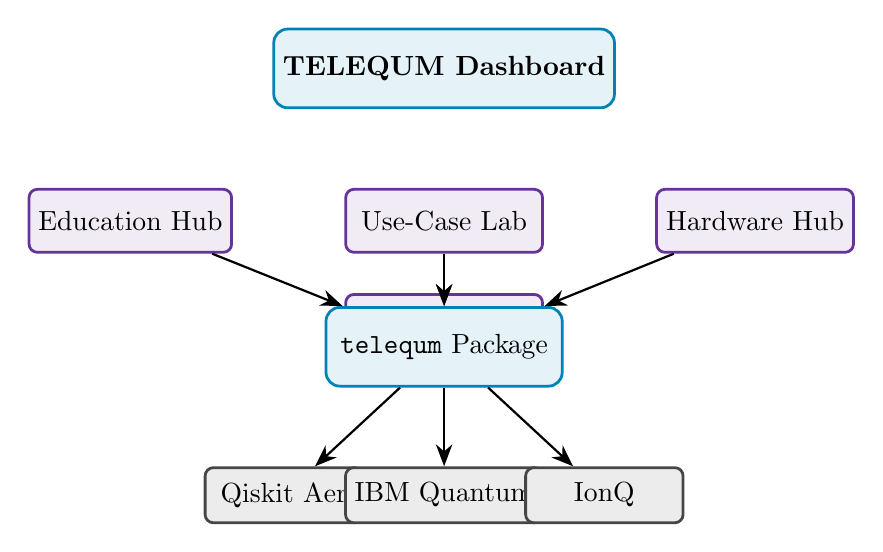
\begin{tikzpicture}[
    node distance=1.5cm,
    box/.style={rectangle, draw=ericssonblue, line width=1pt, 
                minimum width=3cm, minimum height=1cm, 
                rounded corners=5pt, fill=ericssonblue!10},
    module/.style={rectangle, draw=quantumpurple, line width=1pt,
                   minimum width=2.5cm, minimum height=0.8cm,
                   rounded corners=3pt, fill=quantumpurple!10},
    backend/.style={rectangle, draw=telecomgray, line width=1pt,
                    minimum width=2cm, minimum height=0.7cm,
                    rounded corners=3pt, fill=telecomgray!10},
    arrow/.style={-{Stealth[scale=1.2]}, thick}
]

% Frontend
\node[box] (frontend) {\textbf{TELEQUM Dashboard}};

% Modules
\node[module, below left=1cm and 0.5cm of frontend] (edu) {Education Hub};
\node[module, below=1cm of frontend] (lab) {Use-Case Lab};
\node[module, below right=1cm and 0.5cm of frontend] (hw) {Hardware Hub};
\node[module, below=0.5cm of lab] (moon) {Moonshot};

% Core Package
\node[box, below=2.5cm of frontend] (core) {\texttt{telequm} Package};

% Backends
\node[backend, below left=1cm and -0.5cm of core] (sim) {Qiskit Aer};
\node[backend, below=1cm of core] (ibm) {IBM Quantum};
\node[backend, below right=1cm and -0.5cm of core] (ionq) {IonQ};

% Arrows
\draw[arrow] (edu) -- (core);
\draw[arrow] (lab) -- (core);
\draw[arrow] (hw) -- (core);
\draw[arrow] (moon) -- (core);
\draw[arrow] (core) -- (sim);
\draw[arrow] (core) -- (ibm);
\draw[arrow] (core) -- (ionq);

\end{tikzpicture}
\end{center}

% ============================================
% ENTERPRISE READINESS
% ============================================
\section{Enterprise Readiness Features}

\subsection{CI/CD Pipeline (GitHub Actions)}

\begin{lstlisting}[language=yaml, caption={.github/workflows/ci.yml}]
name: TELEQUM CI
on: [push, pull_request]

jobs:
  test:
    runs-on: ubuntu-latest
    strategy:
      matrix:
        python-version: ['3.10', '3.11', '3.12']
    steps:
      - uses: actions/checkout@v4
      - uses: actions/setup-python@v5
        with:
          python-version: ${{ matrix.python-version }}
      - run: pip install -e ".[dev]"
      - run: pytest tests/ -v --cov=telequm
      - run: ruff check telequm/
      - run: mypy telequm/
\end{lstlisting}

\subsection{Testing Strategy}

\begin{tabular}{lp{8cm}}
\toprule
\textbf{Test Type} & \textbf{Scope} \\
\midrule
Unit Tests & QAOA, VQE, QML algorithm correctness \\
Integration Tests & Notebook execution via \texttt{pytest-nbmake} \\
Smoke Tests & Dashboard startup and page loads \\
\bottomrule
\end{tabular}

\subsection{Documentation Standards}

\begin{itemize}
    \item \textbf{API Documentation}: Auto-generated via Sphinx/MkDocs
    \item \textbf{README}: Acquisition-ready positioning (see Section~\ref{sec:readme})
    \item \textbf{CONTRIBUTING.md}: Clear PR process and code standards
    \item \textbf{ARCHITECTURE.md}: System design for technical evaluators
\end{itemize}

% ============================================
% MOONSHOT MODULE
% ============================================
\section{Moonshot Module: Deep Investigation}

\subsection{Vision}
Position TELEQUM as the \textbf{only} open-source platform investigating next-generation propulsion and anti-gravity simulation as high-compute optimization problems.

\subsection{Technical Approach}
\begin{enumerate}
    \item \textbf{Problem Formulation}: Model propulsion optimization as a Quadratic Unconstrained Binary Optimization (QUBO) problem
    \item \textbf{VQE Application}: Use Variational Quantum Eigensolver to find ground state energy configurations
    \item \textbf{QAOA Optimization}: Apply Quantum Approximate Optimization Algorithm for trajectory optimization
    \item \textbf{QML Integration}: Quantum Machine Learning for predictive modeling
\end{enumerate}

\subsection{Research Integration}
\begin{itemize}
    \item Connect with academic partners (Saraya Hamra University)
    \item Publish findings via IEEE/IET channels
    \item Create demonstration notebooks for stakeholder engagement
\end{itemize}

% ============================================
% README POSITIONING
% ============================================
\section{Acquisition-Ready README}
\label{sec:readme}

\subsection{Key Messaging}

\begin{quote}
\textit{``TELEQUM is the bridge between telecom legacy systems and quantum futures. We provide ICT engineers with the tools, education, and industrial simulators needed to integrate quantum computing into real-world telecommunications infrastructure.''}
\end{quote}

\subsection{Value Proposition Sections}

\begin{enumerate}
    \item \textbf{For Telecom Operators}: ROI metrics, migration pathways, PQC readiness
    \item \textbf{For ICT Engineers}: Zero-to-Hero curriculum, hands-on notebooks
    \item \textbf{For Enterprise}: Documentation standards, CI/CD, testing coverage
    \item \textbf{For Investors/Acquirers}: Unique positioning, market opportunity, team credentials
\end{enumerate}

% ============================================
% IMPLEMENTATION TIMELINE
% ============================================
\section{Implementation Timeline}

\begin{longtable}{lp{3cm}p{6cm}}
\toprule
\textbf{Phase} & \textbf{Duration} & \textbf{Deliverables} \\
\midrule
\endhead
Phase 1: Infrastructure & 2--3 days & \texttt{pyproject.toml}, package structure, core modules \\
Phase 2: Legacy Preservation & 1 day & Move all current files to \texttt{v1\_legacy/} \\
Phase 3: Notebooks & 2--3 days & Reorganized curriculum, refactored imports \\
Phase 4: Dashboard & 3--5 days & Streamlit app with 4 main pages \\
Phase 5: Enterprise & 2--3 days & CI/CD, tests, documentation \\
Phase 6: Moonshot & Ongoing & Research module with VQE/QAOA \\
\midrule
\textbf{Total MVP} & \textbf{10--14 days} & Acquisition-ready v2.0 \\
\bottomrule
\end{longtable}

% ============================================
% SUCCESS METRICS
% ============================================
\section{Success Metrics}

\subsection{Technical Metrics}
\begin{itemize}
    \item 100\% notebook execution pass rate
    \item $>$80\% test coverage on core package
    \item All CI checks green on every PR
\end{itemize}

\subsection{Business Metrics}
\begin{itemize}
    \item README clearly articulates ROI for telecom operators
    \item Dashboard demonstrates 3+ industrial use cases
    \item Documentation enables enterprise evaluation in $<$30 minutes
\end{itemize}

\subsection{Community Metrics}
\begin{itemize}
    \item Clear contribution pathway documented
    \item Legacy content accessible and preserved
    \item Professional branding throughout
\end{itemize}

% ============================================
% APPENDIX
% ============================================
\appendix
\section{Current Asset Inventory}

\subsection{IEEE-ComSoc Workshop}
\begin{itemize}
    \item \texttt{Quantum Computing Basics - ComSoc V2.ipynb}
    \item \texttt{Section 1 - Bell State Creation.ipynb}
    \item \texttt{Section 2 - Quantum in Telecommunications.ipynb}
    \item \texttt{Section 3 - Quantum Fourier Transform.ipynb}
    \item \texttt{Section 4 - Phase Control Interference.ipynb}
    \item \texttt{Section 5 - Conclusion Next Steps.ipynb}
\end{itemize}

\subsection{Quantum Computing for 6G and Beyond}
\begin{itemize}
    \item \texttt{04\_1\_6G\_Network\_Optimization\_with\_QAOA.ipynb}
    \item \texttt{04\_2\_6G\_Advanced\_Resource\_Allocation\_with\_VQE.ipynb}
    \item \texttt{04\_3\_6G\_Intelligent\_Beamforming\_with\_QML.ipynb}
    \item \texttt{04\_3.2\_6G\_Intelligent\_Beamforming\_Classical.ipynb}
\end{itemize}

\subsection{QCoffee Corner: The Quantum Heist}
\begin{itemize}
    \item \texttt{Quantum\_Heist\_V1.ipynb} through \texttt{V6.ipynb}
    \item \texttt{Telegram Packets All.json} (70MB --- consider Git LFS)
\end{itemize}

\subsection{Saraya Hamra University}
\begin{itemize}
    \item \texttt{11.ipynb}
    \item \texttt{Beyond\_Bits\_Quantum\_for\_AI\_Engineers.ipynb}
\end{itemize}

% ============================================
% END DOCUMENT
% ============================================
\end{document}
